\chapter{Spacetime and Einstein's Gravity, Gently}
\label{ch:f2}

\section{Gravity is not a pull}

Newton described gravity as a force: the Earth pulls the apple, the Sun
pulls the Earth. His description is astonishingly accurate for slow
objects far from big masses, and Chapter~\ref{ch:f5} will use it freely.
But it leaves a mystery — how does the Sun reach across empty space to
tug on the Earth? — and it fails, measurably, exactly in the situations
this report cares about.

Einstein's 1915 answer, \emph{general relativity}, removes the mystery by
removing the force. In his picture, mass does not pull on distant objects.
Instead, mass changes the shape of \emph{spacetime} — the four-dimensional
fabric of the three space directions plus time — in its neighbourhood, and
objects then simply travel through that reshaped fabric in the straightest
possible lines. The famous slogan, due to John Wheeler, is: \emph{matter
tells spacetime how to curve, and spacetime tells matter how to move.}

A useful (if imperfect) picture is a stretched rubber sheet with a bowling
ball resting in the middle. Marbles rolled across the sheet curve toward
the ball, not because the ball grips them, but because the surface they
travel on slopes. Each marble is doing the most natural thing possible —
going straight ahead on a surface that is not flat. The Earth orbits the
Sun for the same reason: it moves straight ahead through a region of
spacetime that the Sun has curved, and ``straight ahead'' there is a loop.

The straightest possible path through curved spacetime has a name that
appears on nearly every page of Part~II: a \emph{geodesic}. On the Earth's
curved surface, geodesics are the great circles that airliners follow; in
curved spacetime, geodesics are the paths of everything that falls freely
— thrown stones, orbiting planets, and light itself. The entire simulator
described in this report is, at its heart, a machine for computing
geodesics very accurately.

\section{Light bends}

Because light also travels through spacetime, its path also bends where
spacetime curves. The effect is tiny near the Sun — starlight grazing the
solar surface deflects by less than two arcseconds, first measured during
the 1919 eclipse — but near a black hole the bending becomes wild.

Fig.~\ref{fig:trajschw} shows real computed light paths around a
non-spinning black hole, calculated with the same equations the simulator
uses. A ray passing far away bends gently, like the starlight of 1919. A
ray passing closer bends more. And there is a critical aiming distance at
which the bending wins completely: the ray wraps around the hole and can
circle it — light in orbit. Aim any closer and the ray spirals in and is
gone. The dividing line between ``escapes, however bent'' and ``captured''
is what carves out the black-hole \emph{shadow}, the subject of
Chapter~\ref{ch:f3}.

\begin{figure}
\centering
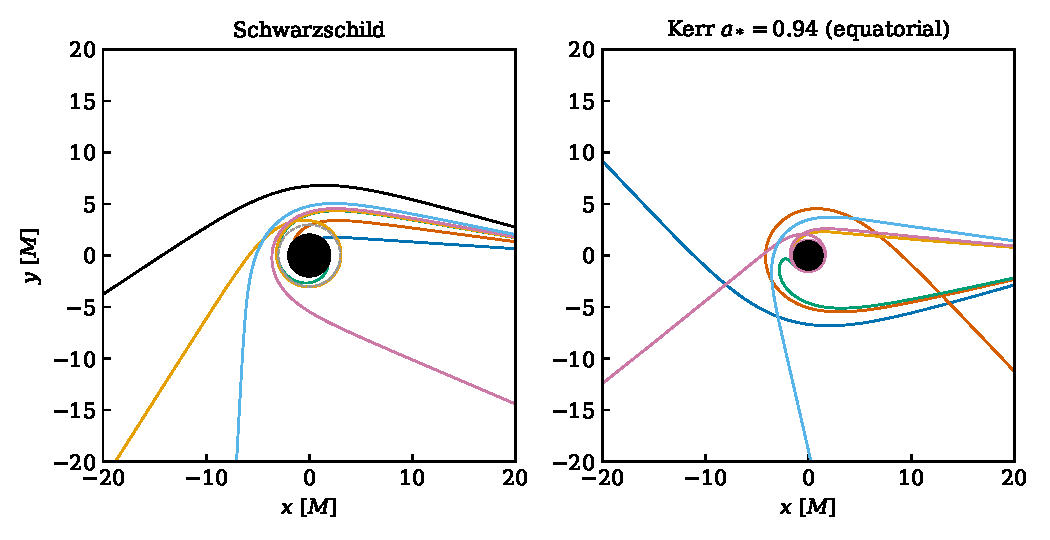
\includegraphics[width=\textwidth]{figures/fig_photon_trajectories.pdf}
\caption{Computed paths of light rays in the equatorial plane of a black
hole, from the simulator's own geodesic integrator. Left: a non-spinning
(Schwarzschild) hole — rays aimed farther out escape with a bend; a
critical ray circles on the dashed photon sphere; closer rays are
captured. Right: a rapidly spinning (Kerr) hole — the spacetime itself
circulates, so rays travelling with the spin behave differently from rays
travelling against it (Chapter~\ref{ch:f3}).}
\label{fig:trajschw}
\end{figure}

This bending also acts as a distorting lens. A black hole with a glowing
disk around it shows you the disk twice over: light from the part of the
disk hidden \emph{behind} the hole is bent up and over the top (and under
the bottom), so the far side appears above and below the dark centre. That
is why the famous images — the Event Horizon Telescope's photographs and
the film \emph{Interstellar}'s Gargantua — have their characteristic
crossed-halo look. Every one of those features appears, for the right
physical reasons, in the renders of Part~III.

\begin{worked}{The 1919 deflection, in two lines}
General relativity gives a compact formula for the bending of a light
ray that passes a mass $m$ at closest distance $r$ (it follows from the
same equations the simulator integrates, Chapter~\ref{ch:geodesics}):
\[
\delta = \frac{4Gm}{c^2 r}.
\]
The combination $Gm/c^2$ — a mass expressed as a length — will follow
us through the whole report; for the Sun it is $1.48$~km. A ray grazing
the solar surface has $r = 696\,000$~km, so
$\delta = 4\times1.48/696\,000 = 8.5\times10^{-6}$~radians. Multiplying
by $206\,265$ (arcseconds per radian) gives $1.75''$ — precisely the
deflection Eddington's expeditions went to measure in 1919, and double
what a na\"ive Newtonian calculation predicts. The factor of two is
pure spacetime curvature: half the bend comes from time running slow,
half from space itself being curved.
\end{worked}

\section{Time runs slow near mass}

Curved spacetime does something with no Newtonian counterpart at all: it
changes the rate of time. Clocks deeper in a gravitational well genuinely
run slower as seen from outside — not because of any mechanical fault, but
because ``one second'' is itself a local quantity, like ``north'', that
depends on where you are.

The effect is real and routine: the satellites of the GPS system carry
clocks about 20\,000~km above the Earth, where time runs faster than at
the ground by about 45 microseconds per day. Uncorrected, satellite
navigation would drift by kilometres within a day. Near a black hole the
same effect grows enormous; at the horizon, an outside observer would see
a falling clock slow to a stop.

\begin{worked}{The GPS correction, by the numbers}
The fractional rate difference between a clock at radius $r_1$ and one
at radius $r_2$ is, to an excellent approximation,
$(Gm/c^2)\,(1/r_1 - 1/r_2)$. For the Earth,
$Gm/c^2 = 4.4$~\emph{millimetres} — the Earth's mass written as a
length. With the ground at $r_1 = 6\,371$~km and the GPS orbit at
$r_2 = 26\,560$~km:
\[
\frac{1}{r_1}-\frac{1}{r_2} = 1.19\times10^{-7}~{\rm m}^{-1},
\qquad
0.0044\times1.19\times10^{-7} = 5.3\times10^{-10}.
\]
Multiply by the $86\,400$ seconds in a day: $46$ microseconds — the
satellite clocks run \emph{fast} by that much, because they sit higher
in the well. (Special relativity's time dilation from orbital speed
works the other way and claws back about $7\,\mu$s, for a net
$39\,\mu$s a day.) Light travels twelve kilometres in $39\,\mu$s:
ignore relativity today and satellite navigation is off by kilometres
by tomorrow.
\end{worked}

For this report the significance is very concrete: when the star S2 dives
to its closest approach to \sgra{}, its light is emitted from slightly
deeper in the black hole's gravitational well, where time runs slower.
Every wave of its light is stretched on the climb out — the wavelength
shifts toward the red. The GRAVITY instrument measured exactly this
\emph{gravitational redshift} in 2018, and reproducing that measurement
from first principles is one of this report's central results
(Chapters~\ref{ch:f4}, \ref{ch:fitting}).

\begin{worked}{S2's slowed clock, on an envelope}
How large is the effect for S2 at closest approach? The fractional
redshift of light climbing out from radius $r$ is roughly $Gm/(c^2 r)$.
For \sgra{}, $Gm/c^2 = 6.35\times10^{9}$~m — half the horizon radius
computed in Chapter~\ref{ch:f1} — and S2's closest approach is
$r \approx 120~{\rm au} = 1.80\times10^{13}$~m:
\[
z_{\rm grav} \approx \frac{6.35\times10^{9}}{1.80\times10^{13}}
= 3.5\times10^{-4}.
\]
A wavelength stretch of $3.5\times10^{-4}$ masquerades, in a
spectrograph, as an extra recession speed of
$3.5\times10^{-4}\times c \approx 106$~km/s. That — about a hundred
km/s of ``impossible'' extra redshift, switching on only around closest
approach — is the size of the signal GRAVITY hunted in 2018, and
Chapter~\ref{ch:fitting} shows our full model reproducing it with no
adjustable amplitude.
\end{worked}

\section{How we know: a century of passed tests}

It is fair to ask why anyone trusts this theory enough to build a
thesis on it. The answer is a hundred years of passed examinations,
each sharper than the last. The 1919 eclipse measurement of bent
starlight (worked above) made the theory famous; the anomalous
43-arcseconds-per-century creep of Mercury's orbit — known and
unexplained for six decades before Einstein — was retro-dicted
exactly, with no adjustable constant. The twentieth century added
laboratory redshift measurements (light climbing a 22-metre tower in
1959), the slowing of radar echoes grazing the Sun, and the patient
20\,000-fold-verified spin-down of the Hulse--Taylor binary pulsar,
which loses orbital energy at precisely the rate gravitational-wave
emission predicts. The twenty-first century has heard those waves
directly (LIGO, 2015) and photographed photon rings (EHT, 2019 and
2022). Every test in this list interrogates a different limb of the
theory — weak field, strong field, static, dynamical — and none has
ever returned a confirmed violation. The measurements this report
reproduces (the S2 redshift and precession, the ring diameter) are
the newest entries in that ledger, and the no-hair test of
Chapter~\ref{ch:nohair} is an attempt to \emph{add} one: the point of
precision reproduction is to build apparatus wherever the theory
could still fail.

\section{What a metric is (without tensors)}

One piece of vocabulary unlocks all of Part~II. To compute anything, we
need coordinates — labels like latitude and longitude that name the points
of spacetime. But coordinates are just names; they do not tell you how
\emph{far apart} two nearby points really are. On the Earth, one degree of
longitude is 111~km at the equator and zero at the pole: the conversion
from coordinate differences to true distances varies from place to place.

The rulebook for that conversion is called the \emph{metric}. Give the
metric the small coordinate steps between two nearby events (a bit of
north--south, a bit of east--west, a bit of time) and it returns the true
separation — including the true amount of elapsed clock time. All of the
curvature of spacetime is encoded in how this rulebook changes from place
to place; slow-running clocks and bending light are both just entries in
the rulebook. Einstein's field equations determine the metric produced by
a given arrangement of mass; for a lone spinning black hole the exact
answer is known and is the famous \emph{Kerr metric}
(Chapters~\ref{ch:f3}, \ref{ch:kerr}), on which this entire simulator is
founded.

When Part~II writes symbols such as $g_{tt}$ or $g_{r r}$, nothing deeper
is meant than ``the entry of the rulebook that converts time-steps (or
radius-steps) into true separations, at this location''.

\begin{termsbox}
\item[Spacetime] Space and time treated as one four-dimensional fabric,
whose shape is what we experience as gravity.
\item[General relativity (GR)] Einstein's theory: mass curves spacetime;
freely falling objects follow the straightest paths in it.
\item[Geodesic] The straightest possible path through curved spacetime;
the track of anything falling freely, including light.
\item[Gravitational lensing] The bending of light by curved spacetime; a
black hole shows the far side of its own disk, bent over the top.
\item[Time dilation] Clocks deeper in a gravitational well run slower;
measurable with GPS satellites and with the star S2.
\item[Gravitational redshift] Light climbing out of a gravitational well
is stretched to longer, redder wavelengths.
\item[Metric] The location-dependent rulebook that converts coordinate
differences into true distances and times; in GR it carries all of
gravity.
\end{termsbox}

\noindent$\rightarrow$ \emph{Full treatment: the Kerr metric in
Chapter~\ref{ch:kerr}; geodesics and their conserved quantities in
Chapter~\ref{ch:geodesics}; the traced light-bending figures in
Chapters~\ref{ch:geodesics} and \ref{ch:shadow}.}
